\chapter{Introduction}
The vision is the human's most important and complex sense, playing a critical role in our orientation in the world \parencite{Hutmacher2019}. However, the health of the retina, an important part of the eye, can be compromised by multiple diseases, that lead to fluid accumulation in it. The characterization of the fluid present in the retina is important to assess the progression of diseases such as age-related macular degeneration (AMD), diabetic macular edema (DME), and macular edema secondary to retinal vein occlusion (RVO) \parencite{Bogunovic2019a}.
\par
AMD affects the macular region of the retina, leading, in later stages, to a significant and permanent loss of central visual acuity, which has a severe impact on the patient's quality of life. In patients with AMD, the formation of new blood vessels can occur, which leak fluid, lipids, and blood into the retina, resulting in the formation of retinal fluid \parencite{Lim2012}. It is one of the leading causes of visual impairment with an expected effect on 300 million people by 2040 \parencite{Mitchell2018}.
\par
In patients with diabetes mellitus, DME represents the most common cause of visual impairment, affecting approximately 150 million people worldwide, as of 2015. It is anticipated that this number will increase as the prevalence of diabetes in developed countries is growing \parencite{Musat2015}. The fluid accumulation is caused by a disruption of the blood-retinal barrier, which allows fluid to accumulate in the intraretinal layers of the macula, resulting in retinal thickening (edema) \parencite{Bhagat2009, Bandello2019}.
\par
Affecting 16 million people worldwide, RVO represents a significant cause of vision loss in older individuals. The occlusion of the retinal vein can result in swelling of the optic disc, which leads to a reduction in visual acuity \parencite{Wong2010}. 
\par
The presence of intraretinal fluid (IRF) is a defining criterion of DME and RVO, while two in every three patients with AMD present this type of fluid. The majority of patients with AMD and 30\% of the patients with DME and RVO have subretinal fluid (SRF). Pigment epithelial detachments (PED) occurs more frequently in patients with AMD \parencite{Bogunovic2019a}.
\par
Therefore, retinal fluids are important for the classification and progression of these diseases, and can be observed through retinal optical coherence tomography (OCT) \parencite{Bogunovic2019a}. OCT is a non-invasive imaging technique that analyzes the light behavior (such as its reflection, absorption, and time-of-flight) to estimate the spatial dimensions of the tissue's structure \parencite{Huang1991}. This allows for \textit{in vivo} visualization of the individual retinal layers within the posterior segment of the eye. An OCT is composed of multiple consecutive cross-sectional 2D images that, when stacked, form a volumetric representation of the posterior segment. Each of these two-dimensional images is referred to as B-scans and an example can be seen in Figure \ref{fig:SegmentedFluidsOCT}. The resolution is sufficiently high to assess the tissue integrity, the retinal layers, and the fluids present \parencite{Drexler2008, Viedma2022}. There are multiple devices used for the acquisition of OCT volumes, resulting in different image attributes across the same technique, such as interslice distance, image quality, and appearance \parencite{Bogunovic2019a}. 
\par
The classification of the fluid is dependent on its location within the retina. There are three different categories: IRF, which is situated in the inner and outer layers of the retina; SRF, positioned between the outer nuclear layer (ONL) and the retinal pigment epithelium (RPE); and PED, which appear beneath the RPE \parencite{Bogunovic2019a}. Figure \ref{fig:SegmentedFluidsOCT} shows the characteristics and positions of these fluids on an OCT B-scan and Figure \ref{fig:RetinalLayers} exhibits the retinal layers in the OCT scan of a healthy patient.
\par
\begin{figure}[!ht]
	\centering
	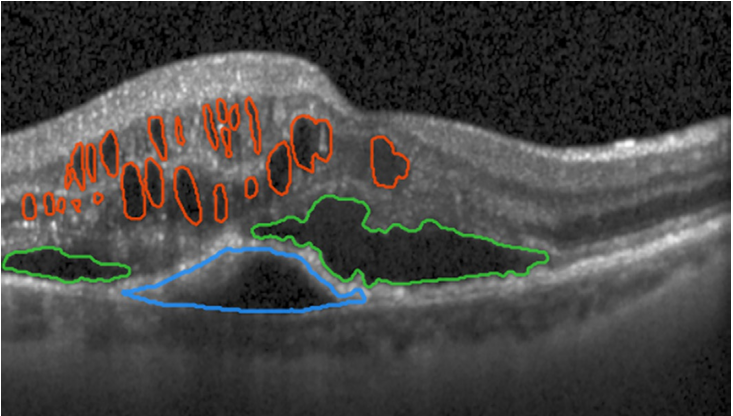
\includegraphics[width=0.75\linewidth]{../figures/SegmentedFluidsOCT.png}
	\caption{The three distinct fluid types on an OCT B-scan: IRF in red, SRF in green, and PED in blue \cite{Bogunovic2019a}.}
	\label{fig:SegmentedFluidsOCT}
\end{figure}
\begin{figure}[!ht]
	\centering
	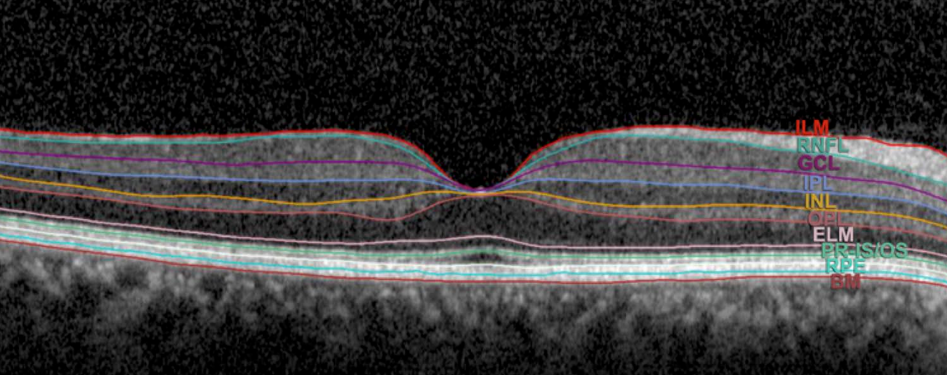
\includegraphics[width=1\linewidth]{../figures/RetinalLayers}
	\caption{OCT scan of the retinal layers \cite{Almonte2020}.}
	\label{fig:RetinalLayers}
	\footnotesize
	\justifying
	BM, Bruch's membrane; ELM, external limiting membrane; GCL, ganglion cell layer; ILM, internal limiting membrane; INL, inner nuclear layer; IPL, inner plexiform layer; ONL, outer nuclear layer; OPL, outer plexiform layer; PR-IS/OS, photoreceptor inner segment/outer segment; RNFL, retinal nerve fibre layer; RPE, retinal pigment epithelium.
\end{figure}
\par
By segmenting the fluids detected in the B-scans, their volume can be estimated and used as a progression marker of the mentioned retinal diseases. However, manual segmentation is laborious, expensive, and prone to bias, which motivates the search for automatic methods \cite{Viedma2022}. 
\par
In OCT imaging, the precision of the estimated volume is not only dependent on the quality of the segmentation, but also on the interslice distance \cite{Lopez2023}. It is seen in other imaging techniques that the performance of the segmentation is improved when the neighboring slices are used as input. Consequently, the reduction in interslice distance and improvement of the resolution along this axis, betters the performance of models that include information from adjacent slices \cite{Selvi2013}. Given that the interslice space is reduced, the estimated segmented volume will also be closer to the real fluid volume.
\par
Considering the previous statements, the dissertation general objective is to conduct an analysis of retinal OCT scans, classifying the retinal fluids in three distinct types (IRF, SRF, and PED) and quantifying their respective volumes. Another important objective is to increase the interslice resolution of the OCT volumes, with the aim of improving the fluid volume estimation. The specific objectives were determined as follows:  
\begin{enumerate}
	\item Develop different 2D deep learning models for multi-class segmentation of retinal fluids (IRF, SRF, and PED) in OCT volumes.
	\item Compare the best performing 2D model with a previously implemented 2.5D model.
	\item Evaluate the performance of the best segmentation model and estimate the volume of each fluid using the masks predicted by it.
	\item Use of a generative model for synthesizing intermediate slices in OCT volumes, generating one or more slices between two real slices to improve the interslice resolution of the volume, while assessing the quality of these generated images.
	\item Investigate the impact of intermediate slices synthesis on the fluid volume estimation by the segmentation models. 
\end{enumerate}
\par
Apart from the ``Introduction", the dissertation is composed of the following chapters: ``Literature Review", ``Methods", ``Results", ``Discussion", and ``Conclusion". In the ``Literature Review" chapter, an analysis is performed on the latest papers in the field of retinal fluid segmentation using 2D deep learning networks, as well as the latest publications on interslice resolution enhancement. The ``Methods" chapter details the selection of the dataset for the experiments performed during the dissertation, alongside with an insightful description of the experiments. In the ``Results" chapter, the results from each experiment are shared, showing the performance of each model in their respective task, while the ``Discussion" chapter explains the performance differences between experiments, comparing them to the literature. Finally, the ``Conclusion" shows the main findings from the experiments performed and suggests directions of further research.
